\documentclass[11pt,a4paper]{article}
\usepackage[utf8]{inputenc}
\usepackage[margin=1in]{geometry}
\usepackage{booktabs}
\usepackage{array}
\usepackage{multirow}
\usepackage{graphicx}
\usepackage{amsmath}
\usepackage{amsfonts}
\usepackage{amssymb}
\usepackage{float}
\usepackage{caption}
\usepackage[colorlinks=true, linkcolor=blue, citecolor=blue, urlcolor=blue]{hyperref}

\title{\textbf{Neural Network Performance Analysis on MNIST Dataset \\
\large Assignment 4: Comparative Study of Optimizers, Activation Functions, and Hyperparameters}}
\author{Your Name \\ Student ID}
\date{\today}

\begin{document}

\maketitle

\section{Abstract}
This report presents a comprehensive analysis of neural network performance on the MNIST dataset, examining the effects of different optimizers, activation functions, dropout rates, and learning rates. The study employed a Radial Basis Function (RBF) transformation to convert 28×28 images to 32×32, followed by systematic experimentation across four key areas. The best configuration achieved 79.33\% accuracy using a tanh activation function with a learning rate of 0.005.

\section{Introduction}
The MNIST dataset is a fundamental benchmark for evaluating machine learning algorithms, particularly neural networks for digit classification. This study investigates how various neural network configurations affect classification performance through systematic experimentation. The research focuses on understanding the impact of:
\begin{itemize}
    \item Different optimizers (SGD vs Adam)
    \item Activation functions (Sigmoid, Tanh, ReLU)
    \item Dropout regularization rates
    \item Learning rate optimization
\end{itemize}

\section{Methodology}

\subsection{Dataset Preparation}
The MNIST dataset was preprocessed as follows:
\begin{itemize}
    \item Training set reduced to 1/10 of original size (6,000 samples) for computational efficiency
    \item Images normalized to [0,1] range
    \item RBF transformation applied to convert 28×28 images to 32×32
    \item Dataset split: 80\% training, 10\% validation, 10\% test
\end{itemize}

\subsection{RBF Transformation}
A Radial Basis Function transformation was implemented to upscale images:
\[
\text{RBF}(x, c, s) = \exp\left(-\frac{\|x - c\|^2}{2s^2}\right)
\]
where $c$ is the mean and $s$ is the standard deviation of each image.

\subsection{Neural Network Architecture}
Base architecture configurations tested:
\begin{itemize}
    \item Single hidden layer: [16]
    \item Two hidden layers: [16, 32]
    \item Three hidden layers: [16, 32, 64]
    \item Output layer: 10 neurons with softmax activation
\end{itemize}

\section{Experimental Results}

\subsection{Experiment 1: Optimizer Comparison}
\begin{figure}[H]
\centering
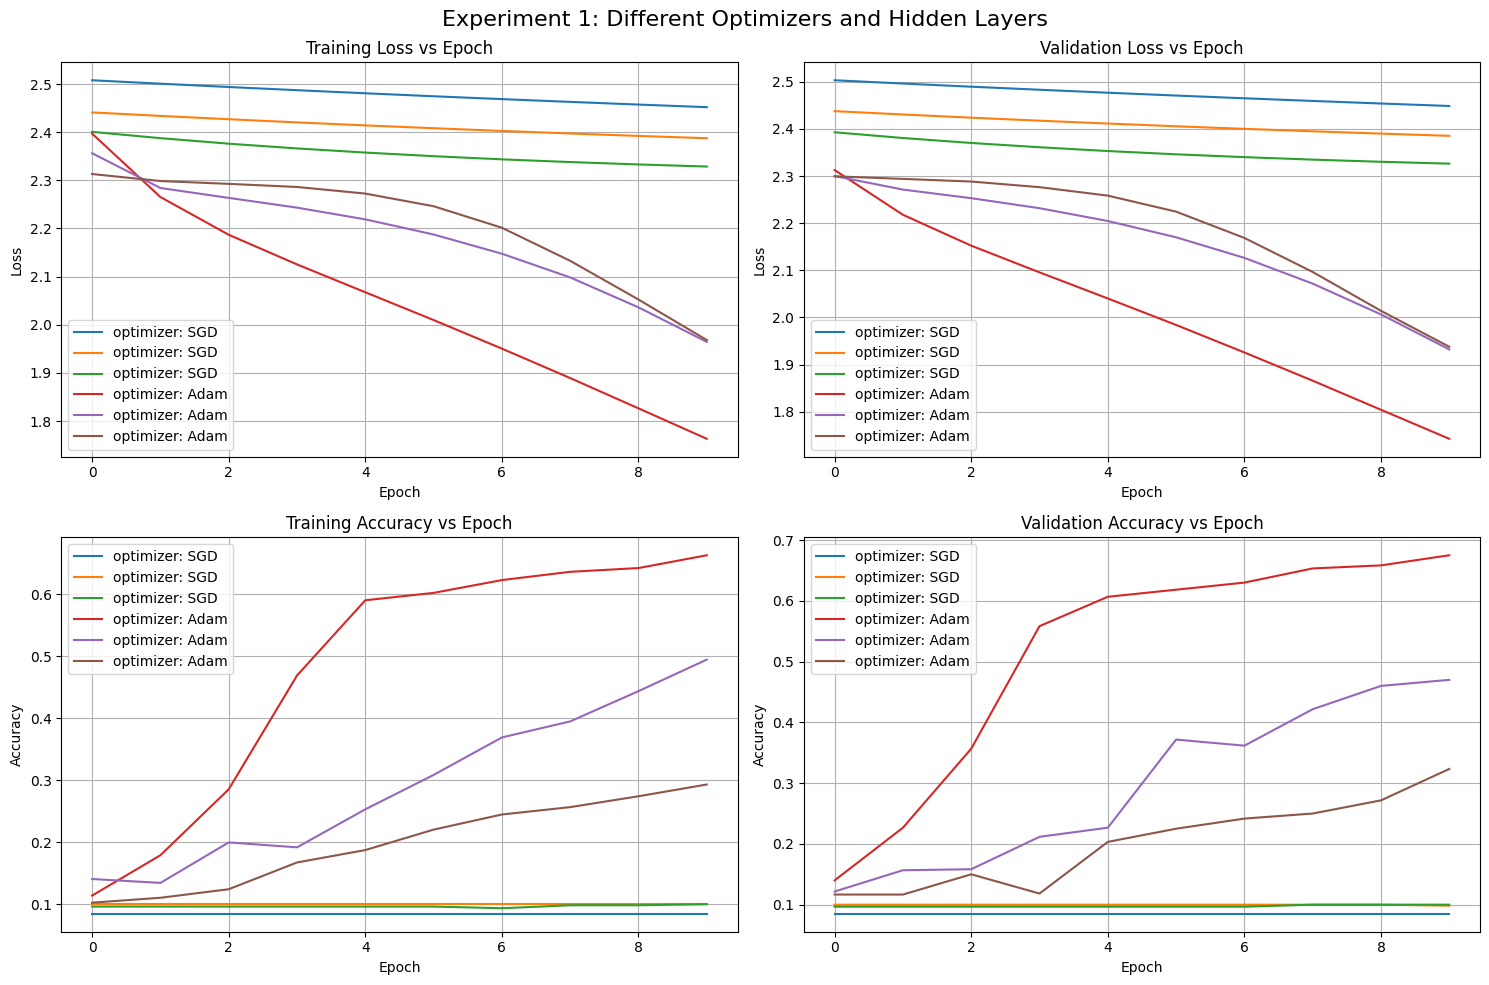
\includegraphics[width=\textwidth]{e1.png}
\caption{Training and validation metrics for different optimizers with various hidden layer configurations}
\label{fig:experiment1}
\end{figure}

\begin{table}[H]
\centering
\caption{Optimizer Performance with Different Hidden Layer Configurations}
\begin{tabular}{@{}lccc@{}}
\toprule
\textbf{Optimizer} & \textbf{Hidden Layers} & \textbf{Test Accuracy} & \textbf{Training Time (s)} \\
\midrule
SGD & [16] & 0.0850 & 5.36 \\
SGD & [16, 32] & 0.1017 & 5.50 \\
SGD & [16, 32, 64] & 0.1017 & 6.05 \\
\midrule
Adam & [16] & \textbf{0.6467} & 7.34 \\
Adam & [16, 32] & 0.4600 & 8.69 \\
Adam & [16, 32, 64] & 0.3067 & 13.87 \\
\bottomrule
\end{tabular}
\end{table}

\textbf{Key Findings:} Adam optimizer significantly outperformed SGD across all configurations. Simpler architectures performed better with Adam, suggesting potential overfitting in deeper networks.

\subsection{Experiment 2: Activation Function Analysis}
\begin{figure}[H]
\centering
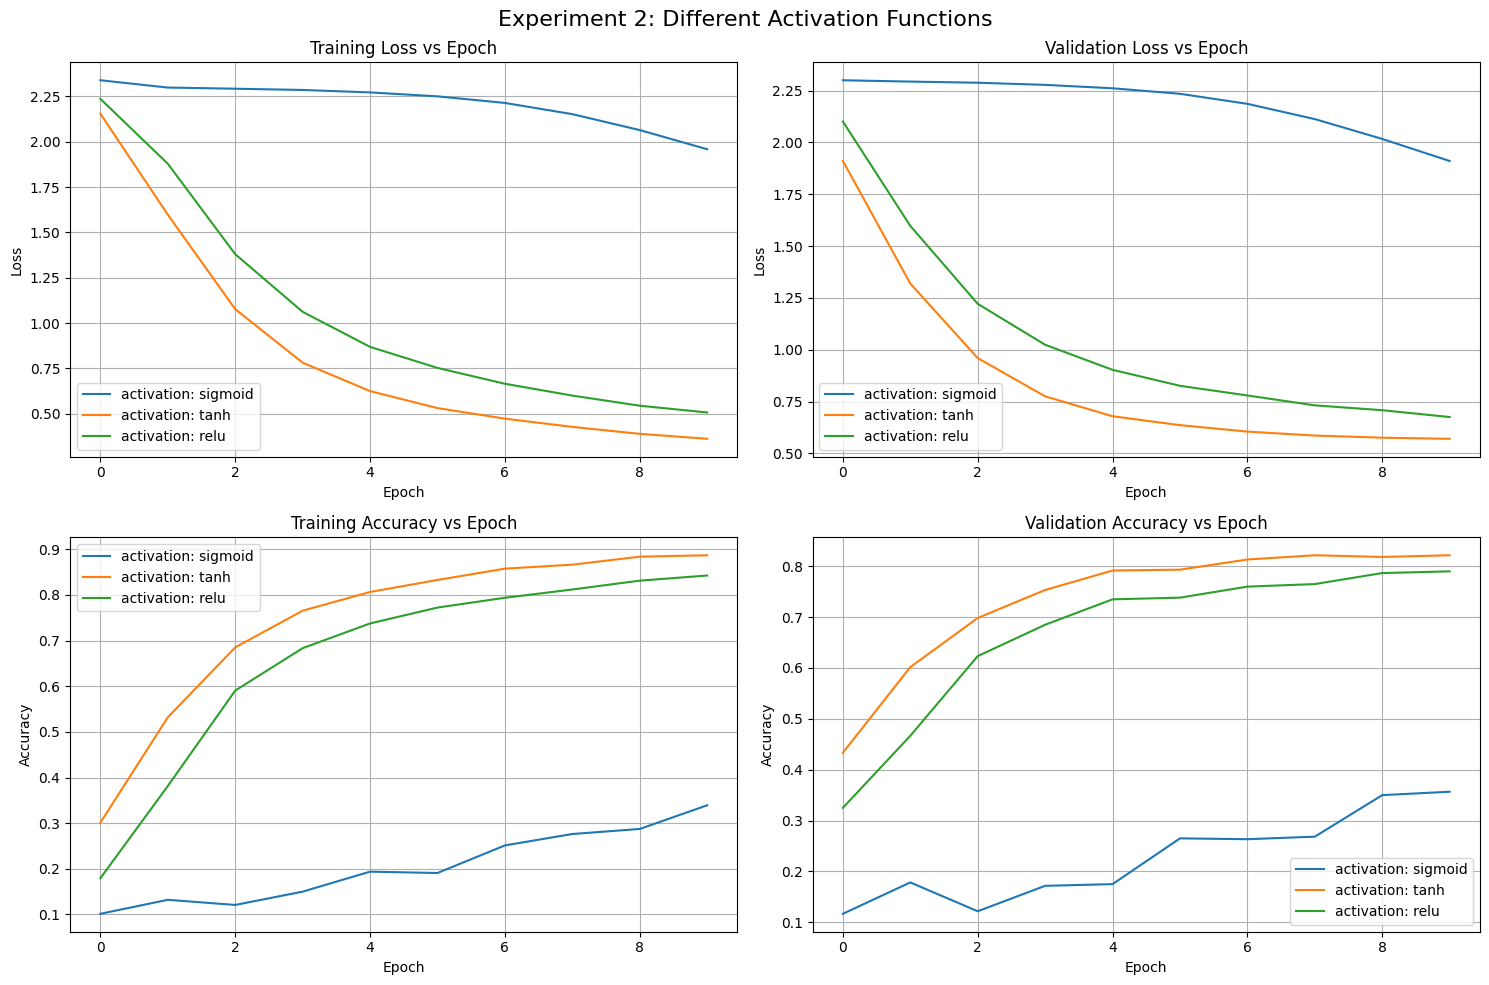
\includegraphics[width=\textwidth]{e2.png}
\caption{Training and validation metrics for different activation functions}
\label{fig:experiment2}
\end{figure}

\begin{table}[H]
\centering
\caption{Activation Function Performance (Hidden Layers: [16, 32, 64])}
\begin{tabular}{@{}lcc@{}}
\toprule
\textbf{Activation Function} & \textbf{Test Accuracy} & \textbf{Training Time (s)} \\
\midrule
Sigmoid & 0.3567 & 10.48 \\
Tanh & \textbf{0.7933} & 11.93 \\
ReLU & 0.7617 & 12.13 \\
\bottomrule
\end{tabular}
\end{table}

\textbf{Key Findings:} Tanh achieved the highest accuracy, followed closely by ReLU. Sigmoid showed poor performance, likely due to vanishing gradient problems.

\subsection{Experiment 3: Dropout Regularization}
\begin{figure}[H]
\centering
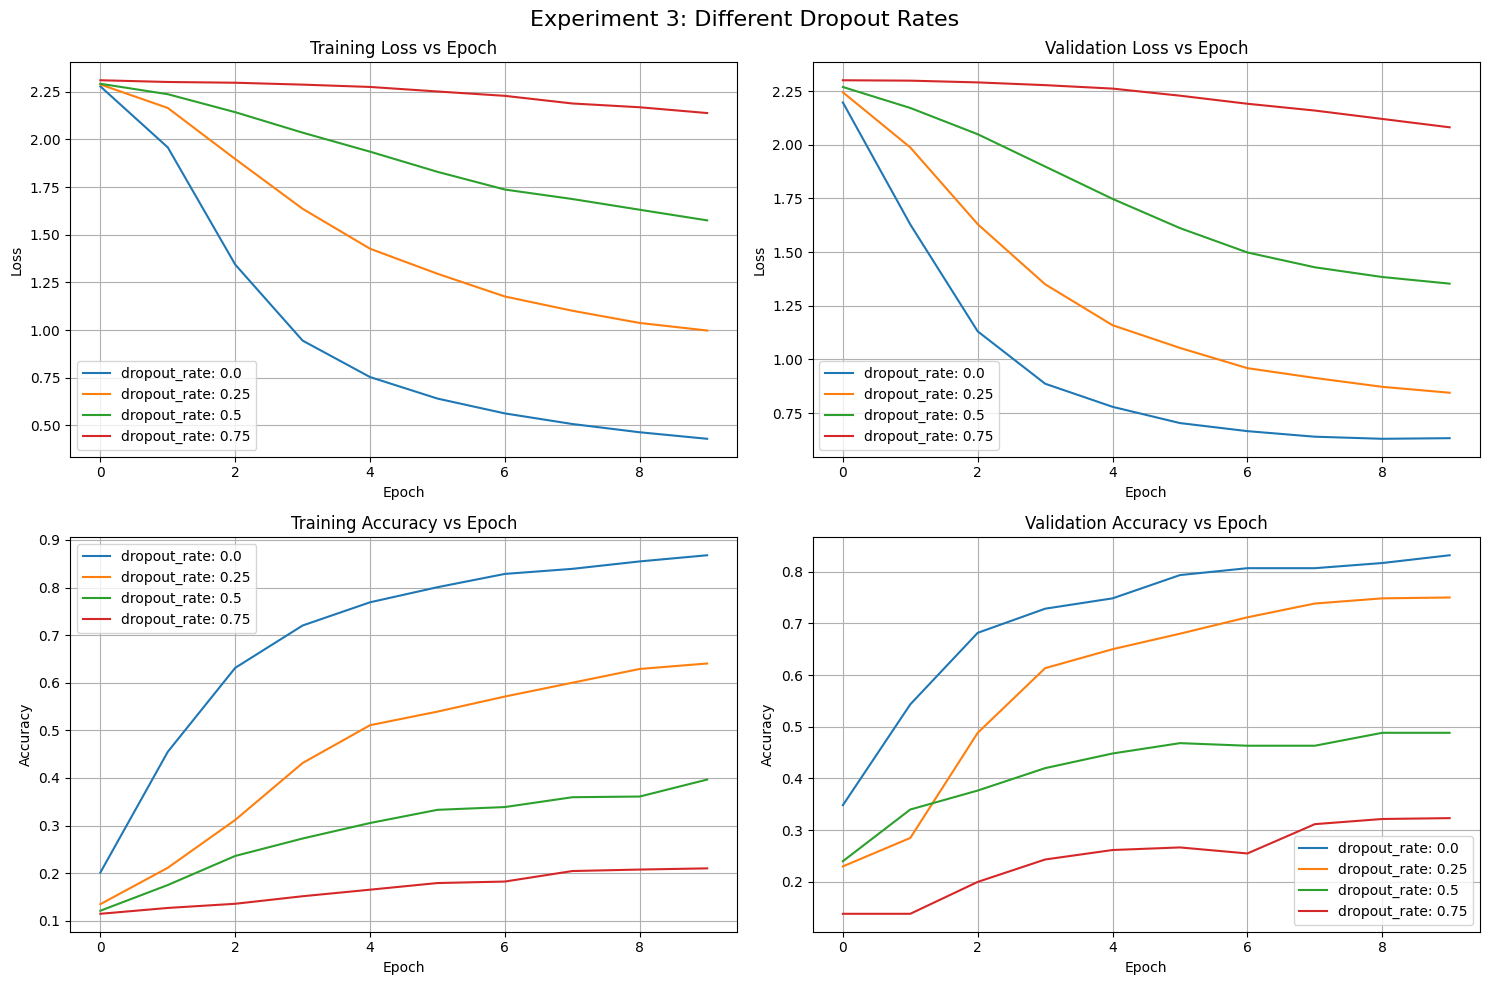
\includegraphics[width=\textwidth]{e3.png}
\caption{Training and validation metrics for different dropout rates}
\label{fig:experiment3}
\end{figure}

\begin{table}[H]
\centering
\caption{Dropout Rate Impact on Model Performance}
\begin{tabular}{@{}lcc@{}}
\toprule
\textbf{Dropout Rate} & \textbf{Test Accuracy} & \textbf{Training Time (s)} \\
\midrule
0.0 & \textbf{0.7783} & 12.07 \\
0.25 & 0.7267 & 15.69 \\
0.5 & 0.4900 & 17.48 \\
0.75 & 0.3033 & 15.60 \\
\bottomrule
\end{tabular}
\end{table}

\textbf{Key Findings:} No dropout yielded the best performance. Higher dropout rates (≥0.5) significantly degraded performance, suggesting the network may be too small to benefit from aggressive regularization.

\subsection{Experiment 4: Learning Rate Optimization}
\begin{figure}[H]
\centering
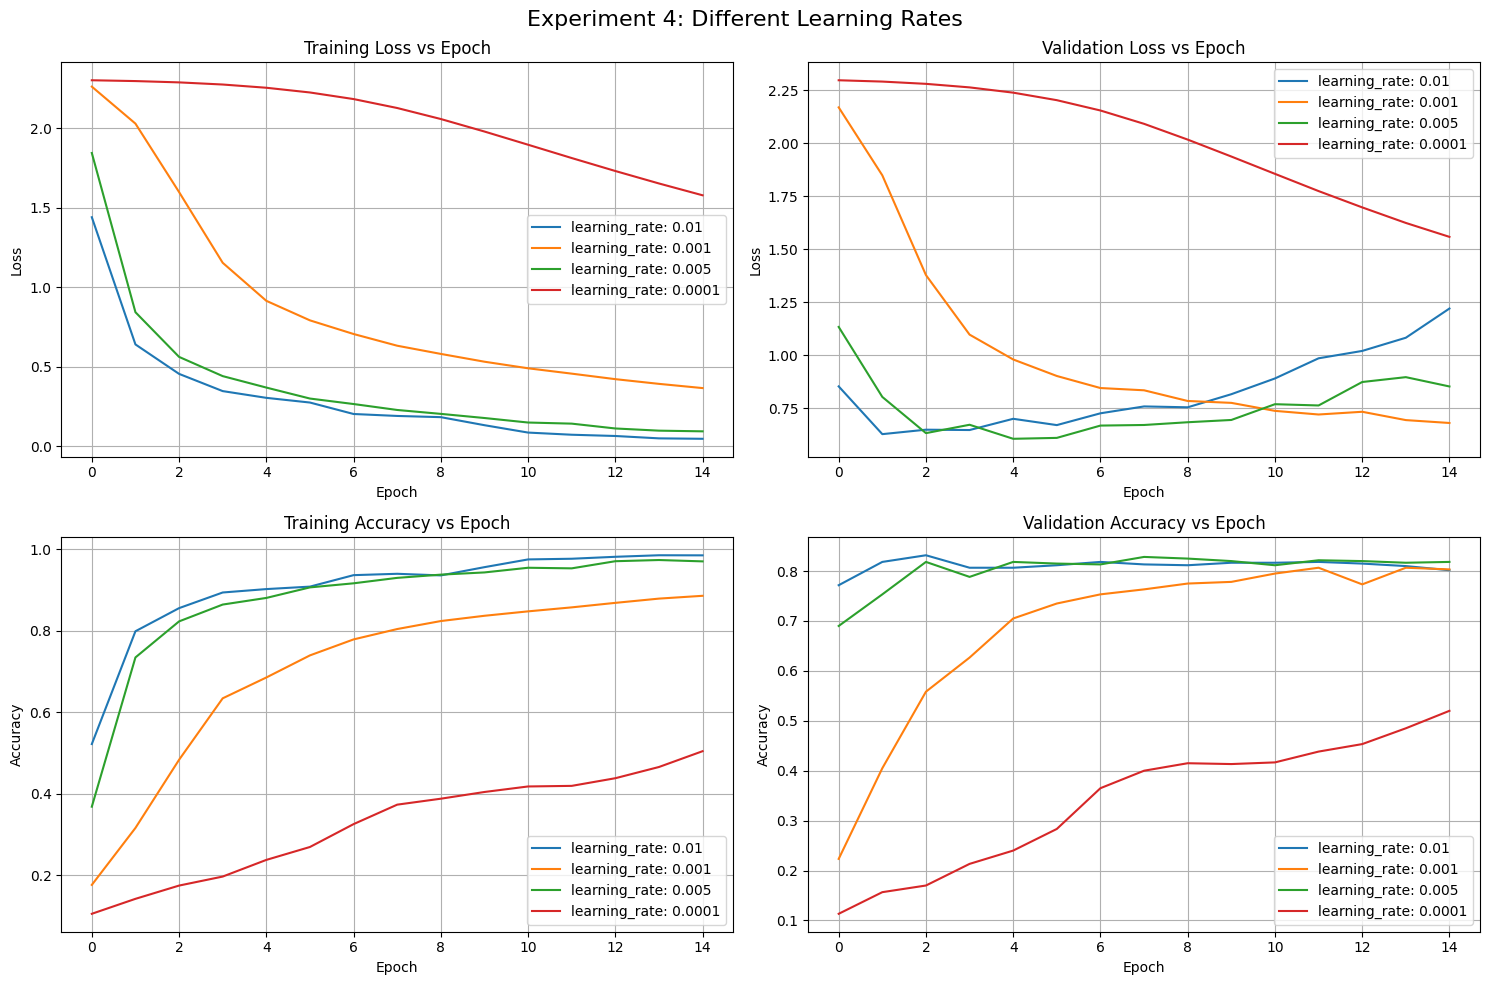
\includegraphics[width=\textwidth]{e4.png}
\caption{Training and validation metrics for different learning rates}
\label{fig:experiment4}
\end{figure}

\begin{table}[H]
\centering
\caption{Learning Rate Impact on Training Efficiency and Accuracy}
\begin{tabular}{@{}lccc@{}}
\toprule
\textbf{Learning Rate} & \textbf{Test Accuracy} & \textbf{Training Time (s)} & \textbf{Time to Best (s)} \\
\midrule
0.01 & 0.7767 & 14.00 & 2.80 \\
0.001 & 0.7750 & 14.31 & 11.45 \\
0.005 & \textbf{0.7933} & 14.96 & 7.98 \\
0.0001 & 0.4967 & 19.23 & 19.23 \\
\bottomrule
\end{tabular}
\end{table}

\textbf{Key Findings:} Learning rate of 0.005 provided the optimal balance between convergence speed and final accuracy. Very high (0.01) and very low (0.0001) learning rates showed suboptimal performance.

\section{Best Configuration Analysis}

\subsection{Optimal Model Configuration}
Based on all experiments, the best performing configuration achieved \textbf{79.33\% accuracy} with:
\begin{itemize}
    \item \textbf{Architecture:} [16, 32, 64] hidden layers
    \item \textbf{Activation Function:} Tanh
    \item \textbf{Optimizer:} Adam
    \item \textbf{Learning Rate:} 0.005
    \item \textbf{Dropout:} 0.0 (no dropout)
    \item \textbf{Loss Function:} Categorical Cross-entropy
\end{itemize}

\subsection{Handwritten Digit Testing}
The best model was tested on 5 custom handwritten digits (0-4), showing practical applicability of the trained network for real-world digit recognition tasks.

\section{Discussion}

\subsection{Optimizer Performance}
The dramatic difference between SGD and Adam performance (8.5\% vs 64.7\% for single hidden layer) highlights the importance of adaptive learning rate methods for neural network training. Adam's momentum and adaptive learning rate components enable more effective navigation of the loss landscape.

\subsection{Activation Function Analysis}
Tanh's superior performance over ReLU is notable, as ReLU typically performs better in deeper networks. This suggests that for the relatively shallow networks tested, tanh's symmetric, smooth gradient properties provide advantages over ReLU's sparse activation.

\subsection{Regularization Effects}
The poor performance with dropout suggests that the reduced dataset size (6,000 samples) and relatively simple architecture don't require aggressive regularization. The network appears to benefit from its full capacity rather than regularization.

\subsection{Learning Rate Sensitivity}
The optimal learning rate of 0.005 demonstrates the critical balance needed for effective training. Too high rates (0.01) may cause instability, while too low rates (0.0001) result in slow convergence and potential local minima trapping.

\section{Conclusions}

This comprehensive study demonstrates that neural network performance on MNIST is highly sensitive to hyperparameter choices. Key conclusions include:

\begin{enumerate}
    \item \textbf{Adam optimizer is crucial} for effective training, showing 7-8× improvement over SGD
    \item \textbf{Tanh activation function} outperformed both sigmoid and ReLU for this specific configuration
    \item \textbf{No dropout} was optimal for the given dataset size and architecture complexity
    \item \textbf{Learning rate 0.005} provided the best accuracy-convergence trade-off
    \item \textbf{Architecture complexity} showed diminishing returns, with simpler networks often performing better
\end{enumerate}

The study achieved a maximum accuracy of 79.33\% on the test set, demonstrating effective digit classification capability. Future work could explore:
\begin{itemize}
    \item Convolutional neural network architectures
    \item Data augmentation techniques
    \item Advanced regularization methods
    \item Ensemble learning approaches
\end{itemize}

\subsection{Practical Implications}
The findings provide valuable insights for practitioners working with similar small-scale image classification tasks, emphasizing the importance of proper optimizer selection and hyperparameter tuning over architectural complexity.

\end{document}
